\chapter{Computer Architecture recalls}

\section{Computer architecture}
It mainly consists of the following elements:
\begin{itemize}
    \item Central Processing Unit (CPU)
    \item Memory Unit
    \item Input/Output Devices( Mass Storage Unit, Keyboard, Display\ldots)
\end{itemize}

Furthermore, the CPU itself consists of three main components:
\begin{itemize}
    \item Control Unit (CU)
    \item Arithmetic/Logic Unit (ALU)
    \item Registers
\end{itemize}

\subsection{Memory}

A computer's memory is where the temporary data and instructions of currently
running programs are located. A computer's memory is also known as Primary
Memory. It is the primary location the CPU uses to retrieve and process data.
It does so very frequently, so the memory must be extremely fast in storing and
retrieving data and instructions.

There are two main types of memory:

\subsubsection{Cache}

memory is usually located within the CPU itself. It runs at the same clock speed as the CPU. 

There are usually three levels of cache memory, depending on their closeness to the CPU core:

\begin{itemize}
        \item Level 1 Cache Usually in kilobytes, the fastest memory
            available, located in each CPU core
        \item Level 2 Cache Usually in megabytes, shared between all CPU cores.
        \item Level 3 Cache Usually in megabytes (Not all CPUs use L3.)
\end{itemize}

\subsubsection{ RAM} located far away from the CPU cores  is much slower than cache
memory. Accessing data from RAM addresses takes many more instructions.

For example, retrieving an instruction from the registers takes only one clock
cycle, and retrieving it from the L1 cache takes a few cycles, while retrieving
it from RAM takes around 200 cyclesa.

In the past, with 32-bit addresses, memory addresses were limited from
0x00000000 to 0xffffffff. This meant that the maximum possible RAM size was 232
bytes, which is only 4 gigabytes, at which point we run out of unique
addresses. With 64-bit addresses, the range is now up to 0xffffffffffffffff,
with a theoretical maximum RAM size of 264 bytes, which is around 18.5 exabytes
(18.5 million terabytes), so we shouldn't be running out of memory addresses
anytime soon.

When a program is run, all of its data and instructions are moved from the
storage unit to the RAM to be accessed when needed by the CPU. 
When a program is closed, its data is removed or made available to re-use from
the RAM.


\subsubsection{Memory Layout of a program}
 The actual layout of a program's in-memory image is left entirely up to the
 operating system, and often the program itself as well. This article focus on
 the concepts of code and data segments of a program and does not take any
 specific platform into account. For a running program both the machine
 instructions (program code) and data are stored in the same memory space. The
 memory is logically divided into text and data segments. Modern systems use a
 single text segment to store program instructions, but more than one segment
 for data, depending upon the storage class of the data being stored there.

 \begin{figure}
  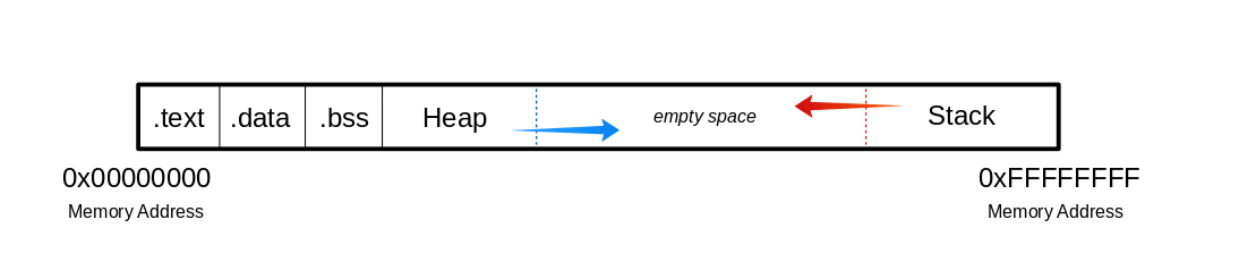
\includegraphics[width=\linewidth]{binary/archi/images/memory-layout.png}
  \caption{Linux memory layout}
  \label{fig:linux-memory-layout}
\end{figure}

{\bf Text Segment}

text segment contains machine code of the compiled
program. The text segment of an executable object file is often read-only
segment that prevents a program from being accidentally modified.

{\bf Data Segments}

Data segment stores program data. This data could be in form of initialized or
uninitialized variables, and it could be local or global. Data segment is
further divided into four sub-data segments (initialized data segment,
uninitialized or \verb+.bss+ data segment, stack, and heap) to store variables
depending upon if they are local or global, and initialized or uninitialized.

{\bf Initialized Data or Data Segment}

Initialized data or simply data segment stores all global, static, constant,
and external variables (declared with \verb+extern+ keyword) that are initialized
beforehand.


{\bf Uninitialized Data or bss Segment}

Contrary to initialized data segment, uninitialized data or \verb+.bss+ segment stores
all uninitialized global, static, and external variables.This section occupies
no actual space in the object file; it is merely a place holder. Object file
formats distinguish between initialized and uninitialized variables for space
efficiency; uninitialized variables do not have to occupy any actual disk space
in the object file.

{\bf Stack Segment}

Stack segment is used to store all local variables and is used for passing
arguments to the functions along with the return address of the instruction
which is to be executed after the function call is over. Local variables have a
scope to the block which they are defined in; they are created when control
enters into the block. Local variables do not appear in data or bss segment.
Also all recursive function calls are added to stack. Data is added or removed
in a last-in-first-out manner to stack. When a new stack frame needs to be
added (as a result of a newly called function), the stack grows downward.

{\bf Heap Segment}
 Heap segment is also part of RAM where dynamically allocated variables are
 stored. 

The stack and heap are traditionally located at opposite ends of the process's
virtual address space.

\subsection{IO/Storage}

Finally, we have the Input/Output devices, like the keyboard, the screen, or
the long-term storage unit, also known as Secondary Memory. The processor can
access and control IO devices using Bus Interfaces, which act as 'highways' to
transfer data and addresses, using electrical charges for binary data.

Each Bus has a capacity of bits it can carry simultaneously. This usually is a multiple of 4-bits, ranging up to 128-bits. Bus interfaces are also usually used to access memory and other components outside the CPU itself. 

Unlike primary memory the storage unit stores permanent data.

The storage unit is the slowest to access. 

\section{CPU architecture}

The Central Processing Unit (CPU) is the main processing unit within a
computer. 

The CPU contains both :
\begin{itemize}
    \item the {\bf Control Unit (CU)}in charge of moving and controlling data
    \item the {\bf Arithmetic/Logic Unit (ALU)}in charge of performing various
        arithmetics and logical calculations as requested by a program through
        the assembly instructions.
\end{itemize}

The manner in which and how efficiently a CPU processes its instructions
depends on its {\bf Instruction Set Architecture (ISA)}. There are multiple
ISA's in the industry, each having its way of processing data:
\begin{itemize}
    \item {\bf RISC} architecture: ased on processing more simple instructions, which takes more cycles, but each cycle is shorter and takes less power. 
    \item {\bf CISC} architecture is based on fewer, more complex instructions, which
        can finish the requested instructions in fewer cycles, but each
        instruction takes more time and power to be processed.
\end{itemize}

\subsection{Clock Speed \& Clock Cycle}

Each CPU has a clock speed that indicates its overall speed. Every tick of the
clock runs a clock cycle that processes a basic instruction, such as fetching
an address or storing an address. Specifically, this is done by the CU or AU.

The frequency in which the cycles occur is counted is cycles per second
(Hertz). If a CPU has a speed of 3.0 GHz, it can run 3 billion cycles every
second (per core).

 \begin{figure}
  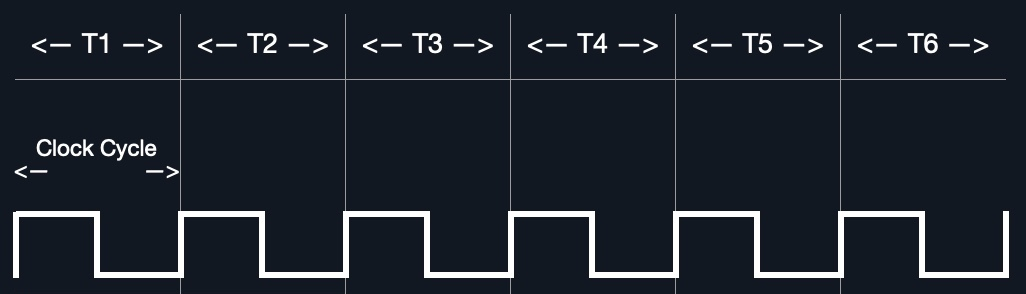
\includegraphics[width=\linewidth]{binary/archi/images/assembly_clock_cycle_0.jpg}
  \caption{Clock cycle}
  \label{fig:clock_cycle_O}
\end{figure}

Modern processors have a multi-core design, allowing them to have multiple
cycles at the same time.


\subsection{Instruction Cycle}
An Instruction Cycle is the cycle it takes the CPU to process a single machine
instruction. An instruction cycle consists of four stages:
\begin{itemize}
    \item Fetch: Takes the next instruction's address from the {\bf Instruction
        Address Register (IAR)}.
    \item Decode: Takes the instruction from the IAR, and decodes it from
        binary to see what is required to be executed.
    \item Execute: Fetch instruction operands from register/memory, and process
        the instruction in the ALU or CU.
    \item Store: Store the new value in the destination operand.
\end{itemize}

Each Instruction Cycle takes multiple clock cycles to finish, depending on the
CPU architecture and the complexity of the instruction. Once a single
instruction cycle ends, the CU increments to the next instruction and runs the
same cycle on it, and so on.

 \begin{figure}
  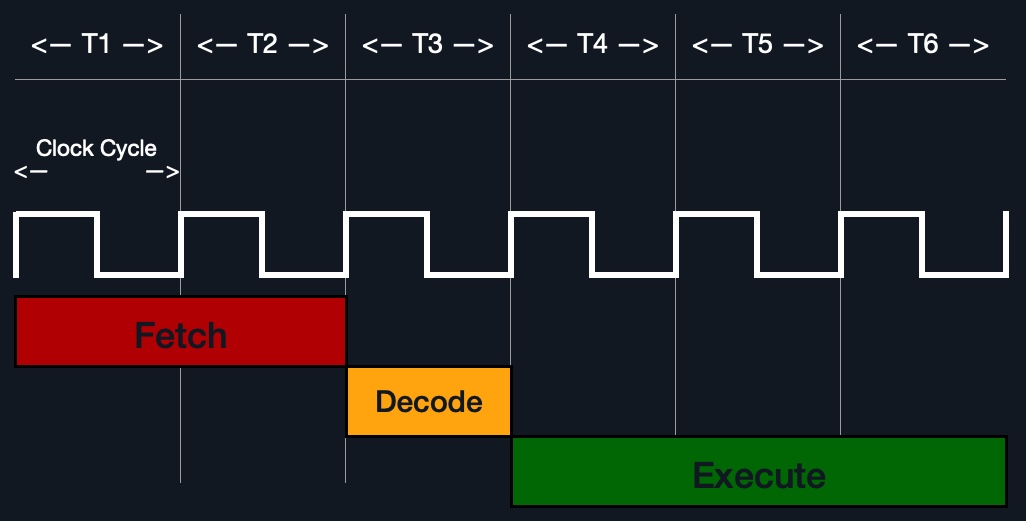
\includegraphics[width=\linewidth]{binary/archi/images/assembly_clock_cycle_1.jpg}
  \caption{Instruction cycle}
  \label{fig:clock_cycle_1}
\end{figure}


In the past, processors used to process instructions sequentially, so they had
to wait for one instruction to finish to start the next. On the other hand,
modern processors can process multiple instructions in parallel by having
multiple instruction/clock cycles running at the same time. This is made
possible by having a multi-thread and multi-core design.

 \begin{figure}
  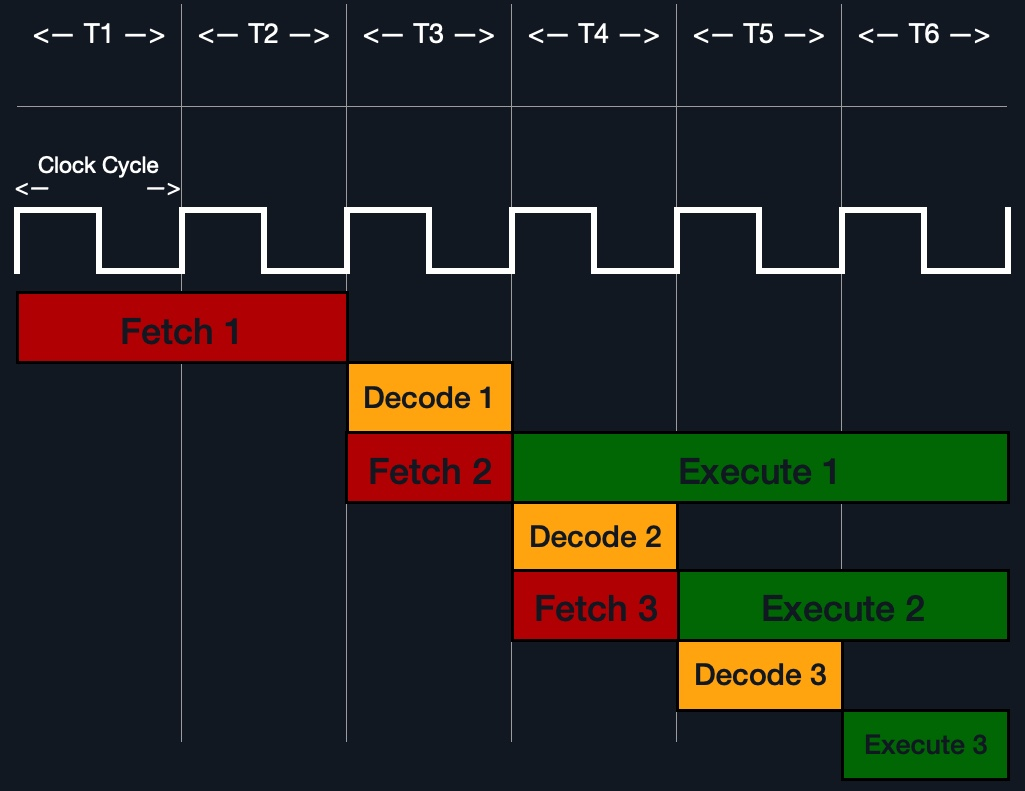
\includegraphics[width=\linewidth]{binary/archi/images/assembly_clock_cycle_2.jpg}
  \caption{Multi-thread instruction cycle}
  \label{fig:clock_cycle_2}
\end{figure}

\subsection{Processor Specific}

Each processor type has a different low-level assembly language
architecture known as {\bf Instruction Set Architectures (ISA)}.

Furthermore, a single Instruction Set Architecture may have several syntax
interpretations for the same assembly code. The instruction written as
\verb+add rax, 1+ with Intel syntax, and written as \verb+addb $0x1,%rax+ with
AT\&T syntax.

As we can see, even though we can tell that both instructions are similar and
do the same thing, their syntax is different, and the locations of the source
and destination operands are swapped as well. Still, both codes assemble the
same machine code and perform the same instruction.



So, each processor type has its Instruction Set Architectures, and each
architecture can be further represented in several syntax formats.

in linux \verb+lscpu+ provide information on the the architecture:
\begin{verbatim}
$ lscpu

Architecture:                    x86_64
CPU op-mode(s):                  32-bit, 64-bit
Byte Order:                      Little Endian

<SNIP>
\end{verbatim}

As we can see in the above output, the CPU architecture is \verb+x86_64+, and
supports 32-bit and 64-bit. The byte order is {\bf Little Endian}. 


\section{Instruction set architectures}
An Instruction Set Architecture (ISA) specifies the syntax and semantics of the
assembly language on each architecture. It is not just a different syntax but
is built in the core design of a processor, as it affects the way and order
instructions are executed and their level of complexity. ISA mainly consists of
the following components:

\begin{itemize}
    \item  Instructions: the instruction to be processed in the {\bf opcode
        operand\_list format}. There are usually 1,2, or 3 comma-separated
    operands \verb+add rax, 1+ \ldots)
    \item  Registers: Used to store operands, addresses, or instructions
        temporarily (\verb+rax, rsp, rip+)
    \item  Memory Addresses: The address in which data or instructions are
        stored. May point to memory or registers 
        (\verb+0xffffffffaa8a25ff, 0x44d0, $rax+)
    \item  Data Types:  The type of stored data (byte, word,\ldots).
\end{itemize}

These are the main components that distinguish different ISA's and assembly languages. 

There are two main Instruction Set Architectures that are widely used:

\begin{itemize}
    \item Complex Instruction Set Computer (CISC) - Used in Intel and AMD
        processors in most computers and servers.
    \item Reduced Instruction Set Computer (RISC) - Used in ARM and Apple
        processors, in most smartphones, and some modern laptops.
\end{itemize}

Let us see the pros and cons of each and the main differences between them.

\subsection{CISC}

The CISC architecture was one of the earliest ISA's ever developed. As its name
suggests, the CISC architecture favors more complex instructions to be run at a
time to reduce the overall number of instructions. This is done to rely as much
as possible on the CPU by combining minor instructions into more complex
instructions.

For example, suppose we were to add two registers with the \verb+add rax, rbx+
instruction. In that case, a CISC processor can do this in a single
'Fetch-Decode-Execute-Store' instruction cycle, without having to split it into
multiple instructions to fetch \verb+rax+, then fetch \verb+rbx+, then add
them, and then store them in `rax, each of which would take its own
'Fetch-Decode-Execute-Store' instruction cycle.

Two main reasons drove this:
\begin{itemize}
    \item To enable more instructions to be executed at once by designing the
        processor to run more advanced instructions in its core.
    \item In the past, memory and transistors were limited, so it was preferred
        to write shorter programs by combining multiple instructions into one.
\end{itemize}

To enable the processors to execute complex instructions, the processor's
design becomes more complicated, as it is designed to execute a vast amount of
different complex instructions, each of which has its own unit to execute it.

Furthermore, even though it takes a single instruction cycle to execute a
single instruction, as the instructions are more complex, each instruction
cycle takes more clock cycles. This fact leads to more power consumption and
heat to execute each instruction.

\subsection{RISC}

The RISC architecture favors splitting instructions into minor instructions,
and so the CPU is designed only to handle simple instructions. This is done to
relay the optimization to the software by writing the most optimized assembly
code.

For example, the same previous \verb+add r1, r2, r3+ instruction on a RISC
processor would fetch \verb+r2+, then fetch \verb+r3+, add them, and finally
store them in \verb+r1+. Every instruction of these takes an entire
'Fetch-Decode-Execute-Store' instruction cycle, which leads, as can be
expected, to a larger number of total instructions per program, and hence a
longer assembly code.

By not supporting various types of complex instructions, RISC processors only
support a limited number of instructions (~200) compared to CISC processors
(~1500). So, to execute complex instructions, this has to be done through a
combination of minor instructions through Assembly.

On the other hand, an advantage of splitting complex instructions into minor
ones is having all instructions of the same length either 32-bit or 64-bit
long. This enables designing the CPU clock speed around the instruction length
so that executing each stage in the instruction cycle would always take
precisely one machine clock cycle.

The below diagram shows how CISC instructions take a variable amount of clock
cycles, while RISC instructions take a fixed amount: risc vs cisc cycles



 \begin{figure}
  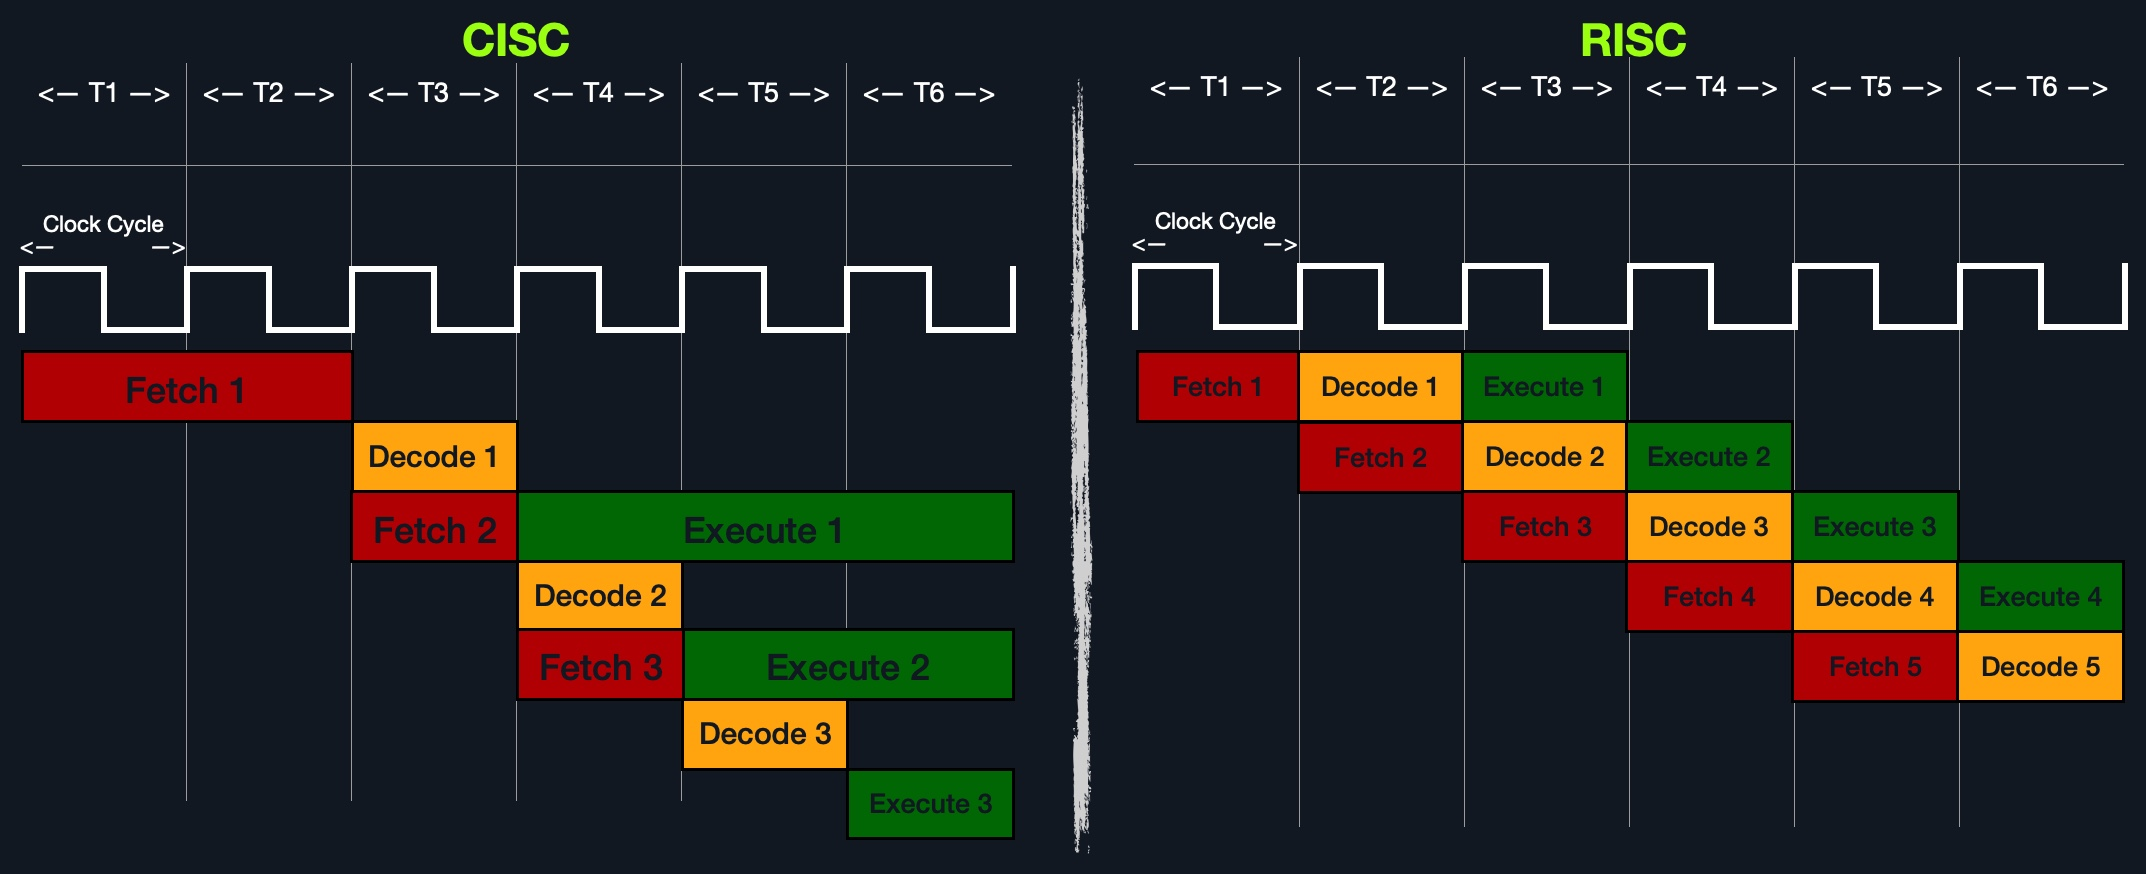
\includegraphics[width=\linewidth]{binary/archi/images/assembly_cisc_risk_cycles.jpg}
  \caption{CISC / RISC cycles}
  \label{fig:assembly_cisc_risk_cycles}
\end{figure}



Executing each instruction stage in a single clock cycle and only executing
simple instructions leads to RISC processors consuming a fraction of the power
consumed by CISC processors, which makes these processors ideal for devices
that run on batteries, like smartphones and laptops.

\subsection{CISC vs. RISC}
In the past, having a longer assembly code due to a larger number of total
instructions per program was a significant disadvantage for RISC processors due
to the limited resources in memory and storage. However, today this is no
longer as big of an issue, as memory and storage are not as expensive and
limited as they used to be in the past.

Furthermore, with new assemblers and compilers writing extremely optimized code
on the software level, RISC processors are becoming faster than CISC
processors, even in executing and processing heavy applications, all while
consuming much less power.

All of this is making RISC processors more common in recent years. RISC may
become the dominant architecture in the upcoming years. But as we speak, the
overwhelming majority of computers and servers we will be pentesting are
running on Intel/AMD processors with the CISC architecture, making learning
CISC assembly our priority. As the basics of all Assembly language variants are
pretty similar, learning ARM Assembly should be more straightforward.

\section{Registers, addresses, and data types}

\subsection{Data Types}

\subsubsection{Bits, bytes, words, double words\ldots}
The x86 architecture supports many types of data sizes, which can be used with
various instructions. The following are the most common data types we will be
using with instructions:
\begin{itemize}
    \item byte 	(8 bits) 	\verb+0xab+
    \item word 	(2 bytes) 	\verb+0xabcd+
    \item double word (dword) 	(4 bytes) 	\verb+0xabcdef12+
    \item quad word (qword) (8 bytes) 	(\verb+0xabcdef1234567890+)
    \item double qwords (16 byts)
\end{itemize}

Whenever we use a variable with a certain data type or use a data type with an
instruction, both operands should be of the same size.

\subsubsection{Endianness}

During load and save operations in registers and memories, the bytes are read
in a different order. This byte order is called endianness. Endianness is
distinguished between the little-endian format and the big-endian format.

Big-endian and little-endian are about the order of valence:
\begin{itemize}
    \item In big-endian, the digits with the highest valence are initially. 
    \item In little-endian, the digits with the lowest valence are at the beginning. 
\end{itemize}

Mainframe processors use the big-endian format, some RISC architectures, minicomputers, and in TCP/IP networks, the byte order is also in big-endian format.

Now, let us look at an example with the following values:

\begin{itemize}
        \item Address: \verb+0xffff0000+
        \item Word: \verb+\xAA\xBB\xCC\xDD+
\end{itemize}

\begin{verbatim}
Memory Address 	0xffff0000 	0xffff0001 	0xffff0002 	0xffff0003
Big-Endian 	        AA 	        BB 	        CC 	        DD
Little-Endian 	    DD 	        CC 	        BB 	        AA
\end{verbatim}

\subsubsection{negative number encoding}

\subsection{Registers}

There are many registers in the x86 architecture, but we will only focus on the
ones necessary for learning basic Assembly and essential for future binary
exploitation.

\subsubsection{Intel 32 bites registers}


{\bf General purpose registers}:
\begin{itemize}
    \item \verb+EAX+ Extended Accumulator Register
    \item \verb+EBX+ Extended Base Register
    \item \verb+ECD+ Extended Counter Register
    \item \verb+EDX+ Extended Data Register
    \item \verb+ESI+ Extended Source Index
    \item \verb+EDI+ Extended Destination Index
    \item \verb+EBP+ Extended Base Pointer
    \item \verb+ESP+ Extended Stack Pointer
\end{itemize}

All the general purpose registers are 32-bit size in Intel’s IA-32 architecture but depending
on their origin and intended purpose, a subset of some of them can be referenced in
assembly.
\begin{verbatim}
32 bits         16 bits         8 bits
EAX             AX              AH / AL
EBX             BX              BH / BL
ECX             CX              CH / CL
EDX             DX              DH / DL
ESI             SI
EDI             DI
EBP             BP
ESP             SP
\end{verbatim}

\verb+AX+ to \verb+SP+ are the 16 bit registers used to reference the 16 least
significant bits in their equivalent 32 bit registers. The eight bit registers
reference the higher and lower eight bits of the 16 bit registers.

{\bf Segment registers}: are used to make segmental distinctions in the binary. We will
approach segments later but in short, the hexadecimal value \verb+0x90+ can
either represent an instruction or a data value. The CPU knows which one thanks
to segment registe.

{\bf Status flag registers}: Flags are tiny bit values that are either set (1)
or not set (0). Each flag represent a status. For example, if the “signed” flag
is set, the value of FF will represent a \verb+-1+ in decimal notation instead
of \verb+255+. Flags are all stored in special flag register, were many one bit
flags are stored at once. The flags are set whenever an operation resulted in
certain state or output. The flags we are most interested in for now are:
\begin{itemize}
        \item Z – zero flag, set when the result of the last operation is zero
            32 bits 16 bits 8 bit
        \item S – signed flag, set to determine if values should be intercepted
            as signed or unsigned
        \item O – overflow flag, set when the result of the last operation
            switches the most significant bit from either F to 0 or 0 to F.
        \item C – carry flag, set when the result of the last operation changes
            the most significant bit
\end{itemize}

{\bf Extended Instruction Pointer (EIP)} The instruction pointer has the same
function in a CPU as the needle had in those old gramophones your grandpa used
to have. It points to the next instruction to be executed.


\subsubsection{Intel 64 bites registers}


{\bf General purpose registers} Sixteen general purpose 64-bit registers:
\begin{itemize}
        \item eight  RAX, RBX, RCX, RDX, RBP, RSI, RDI, and RSP. 
        \item eight are named R8-R15.
\end{itemize}

By replacing the initial \verb+R+ with an \verb+E+ on the first eight
registers, it is possible to access the lower 32 bits (\verb+EAX+ for
\verb+RAX+). 

Similarly, for \verb+RAX+, access to the lower 16 bits is possible by removing
the initial \verb+R+ , and the lower byte of the these by switching the
\verb+X+ for \verb+L+ (\verb+AL+ for \verb+AX+), and the higher byte of the low
16 bits using an \verb+H+ (\verb+AH+ for \verb+AX+). 

The new registers \verb+R8+ to \verb+R15+ can be accessed in a similar manner
like this: \verb+R8+ (qword), \verb+R8D+ (lower dword), \verb+R8W+ (lowest
word), \verb+R8B+ (lowest byte MASM style, Intel style \verb+R8L+). Note there
is no \verb+R8H+


 \begin{figure}
  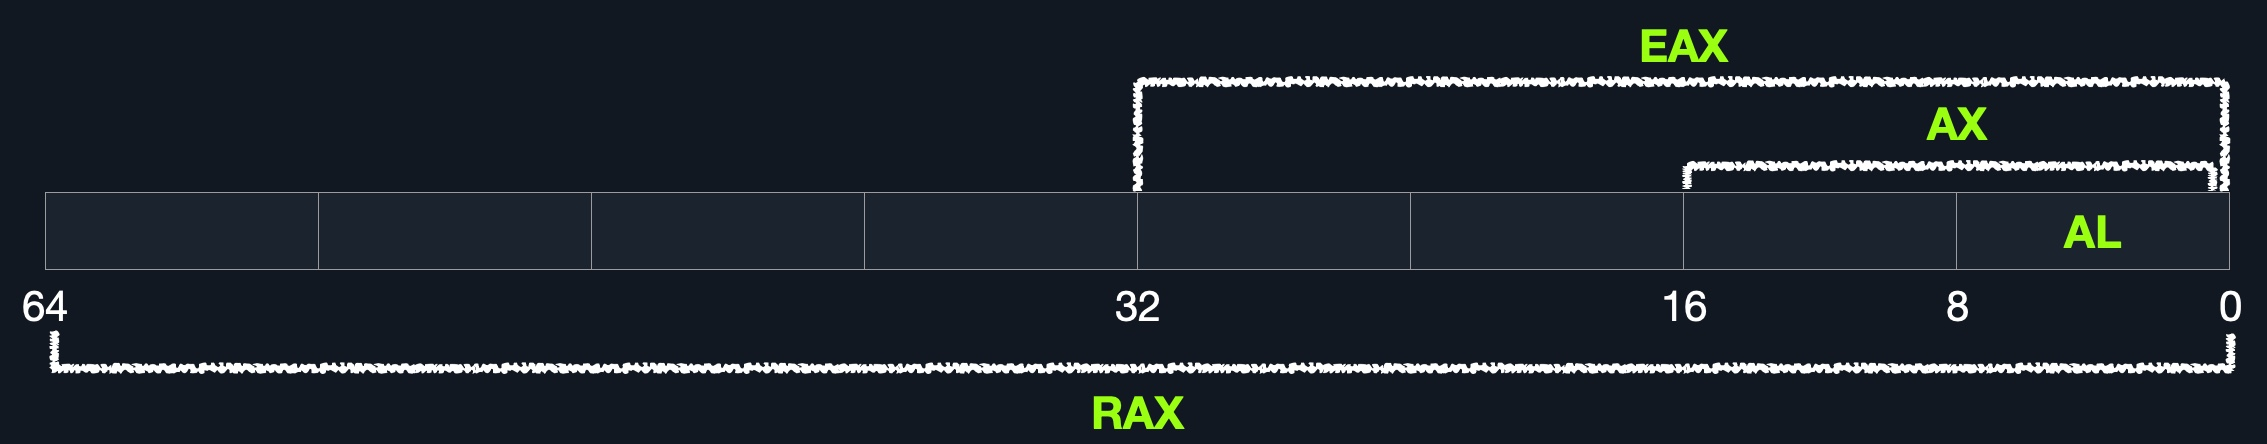
\includegraphics[width=\linewidth]{binary/archi/images/assembly_register_parts.jpg}
  \caption{Registry parts}
  \label{fig:assembly_register_parts}
\end{figure}

\begin{verbatim}
Data/Arguments Registers
    Syscall Number/Return value 	rax 
    Callee Saved 	                rbx 	
    1st arg - Destination operand 	rdi 	
    2nd arg - Source operand  	    rsi 	
    3rd arg 	                    rdx 	
    4th arg - Loop counter 	        rcx 	
    5th arg 	                    r8 	
    6th arg 	                    r9
Pointer Registers
    Base Stack Pointer 	            rbp
    Current/Top Stack Pointer 	    rsp 
    Instruction Pointer 'call only' rip
\end{verbatim}


\subsection{Memory Addresses}

x86 64-bit processors have 64-bit wide addresses that range from \verb+0x0+ to
\verb+0xffffffffffffffff+, so we expect the addresses to be in this range.
However, RAM is segmented into various regions, like the Stack, the heap, and
other program and kernel-specific regions. Each memory region has specific
read, write, execute permissions that specify whether we can read from it,
write to it, or call an address in it.

Whenever an instruction goes through the Instruction Cycle to be executed, the first step is to fetch the instruction from the address it's located at. There are several types of address fetching (i.e., addressing modes) in the x86 architecture:
\begin{verbatim}
Addressing Mode 	Description 	                        Example
Immediate 	        The value is given within               add 2

                    the instruction
Register 	        The register name that holds the        add rax
                    value is given in the instruction

Direct 	            The direct full address is given        call 0xffffffffaa8a25ff
                    in the instruction 	

Indirect 	        A reference pointer is given            call 0x44d000 or call [rax]
                    in the instruction 	     

Stack 	            Address is on top of the stack 	        add rbp
\end{verbatim}

In the above table, lower is slower. The less immediate the value is, the
slower it is to fetch it.

Even though speed isn't our biggest concern when learning basic Assembly, we
should understand where and how each address is located. Having this
understanding will help us in future binary exploitation, with Buffer Overflow
exploits, for example. The same understanding will have an even more
significant implication with advanced binary exploitation, like {\bf ROP} or 
{\bf Heap} exploitation.


